This section shows the screenshot of the web interface used in the user evaluation study (see Section~\ref{subsubsec:quantitative_analysis_of_user_ratings} for the explanation flow).

\vspace{-0.5em}

\begin{figure}[h]
    \centering
    \captionsetup{font=small,skip=4pt}
    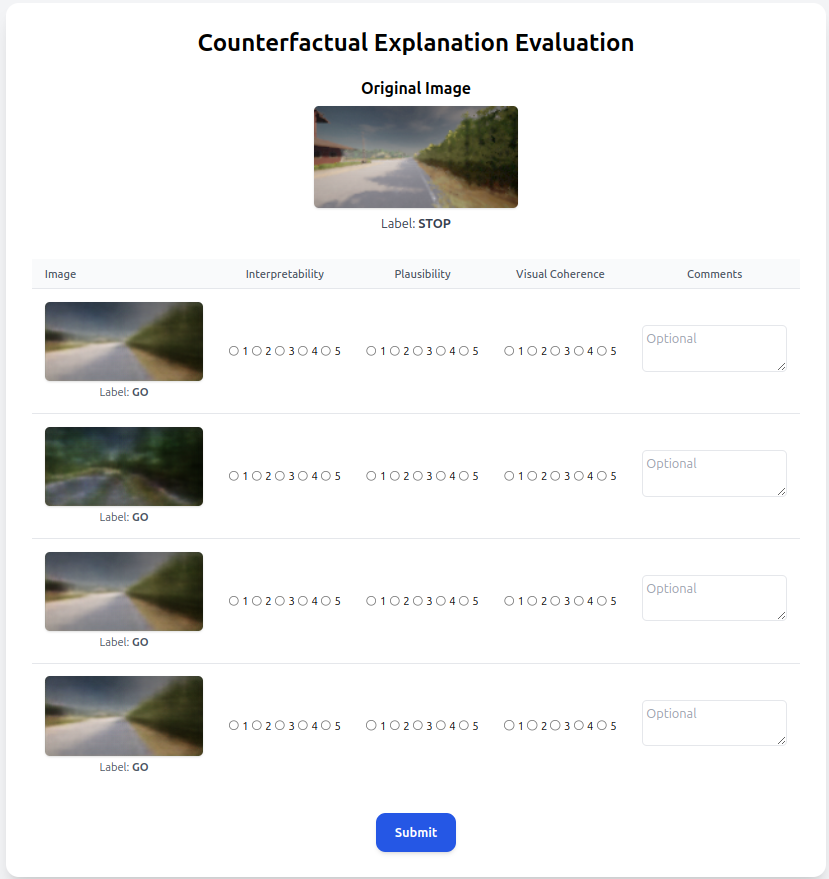
\includegraphics[width=0.68\textwidth]{img/web_app_screenshots/grading.png}
    \caption{Screenshot of the web-based evaluation interface developed for the human user study. The interface presents the original driving scene image (with its predicted label, in this case, \texttt{STOP}) at the top, followed by four counterfactual images—each assigned a predicted label (e.g., \texttt{GO}). For each counterfactual, participants rate interpretability, plausibility, and visual coherence on a 5-point Likert scale. Optional comment boxes are provided for qualitative feedback. This interface implementation is discussed in Section~\ref{subsubsec:quantitative_analysis_of_user_ratings}.}
    \label{fig:app:grading}
\end{figure}


\begin{sidewaysfigure}[htbp]
    \centering
    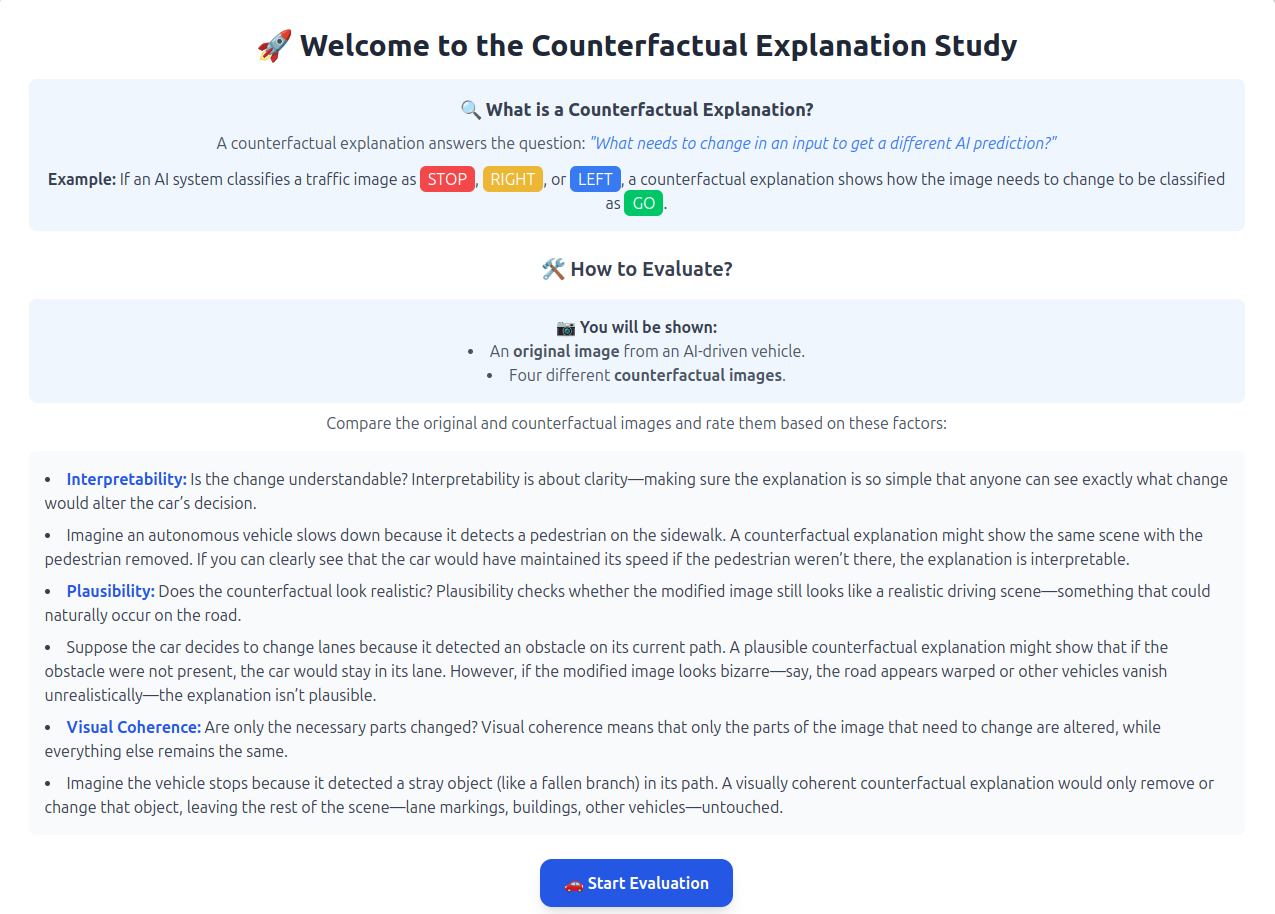
\includegraphics[width=0.78\textwidth]{img/web_app_screenshots/form_ui_info.png}
    \caption{Welcome screen of the user evaluation interface used in the counterfactual explanation study. This introductory page provides participants with a concise overview of the purpose of counterfactual explanations in the context of traffic scene classification (e.g., changing an image classified as \texttt{STOP} to \texttt{GO}). It explains what participants will be shown (an original image followed by four counterfactuals) and outlines the evaluation criteria: Interpretability, Plausibility, and Visual Coherence. Each criterion is defined with examples to ensure a clear and consistent understanding among all evaluators before proceeding to the actual rating task.}
    \label{fig:app:form_ui}
\end{sidewaysfigure}